%\documentclass[11pt,twoside]{mitthesis}
%\usepackage{tikz}
%\usepackage{circuitikz}
%\usepackage{amsmath}
%\begin{document}
\chapter{Hardware}
Block diagram / Schematic
\begin{figure}
  \begin{center}
      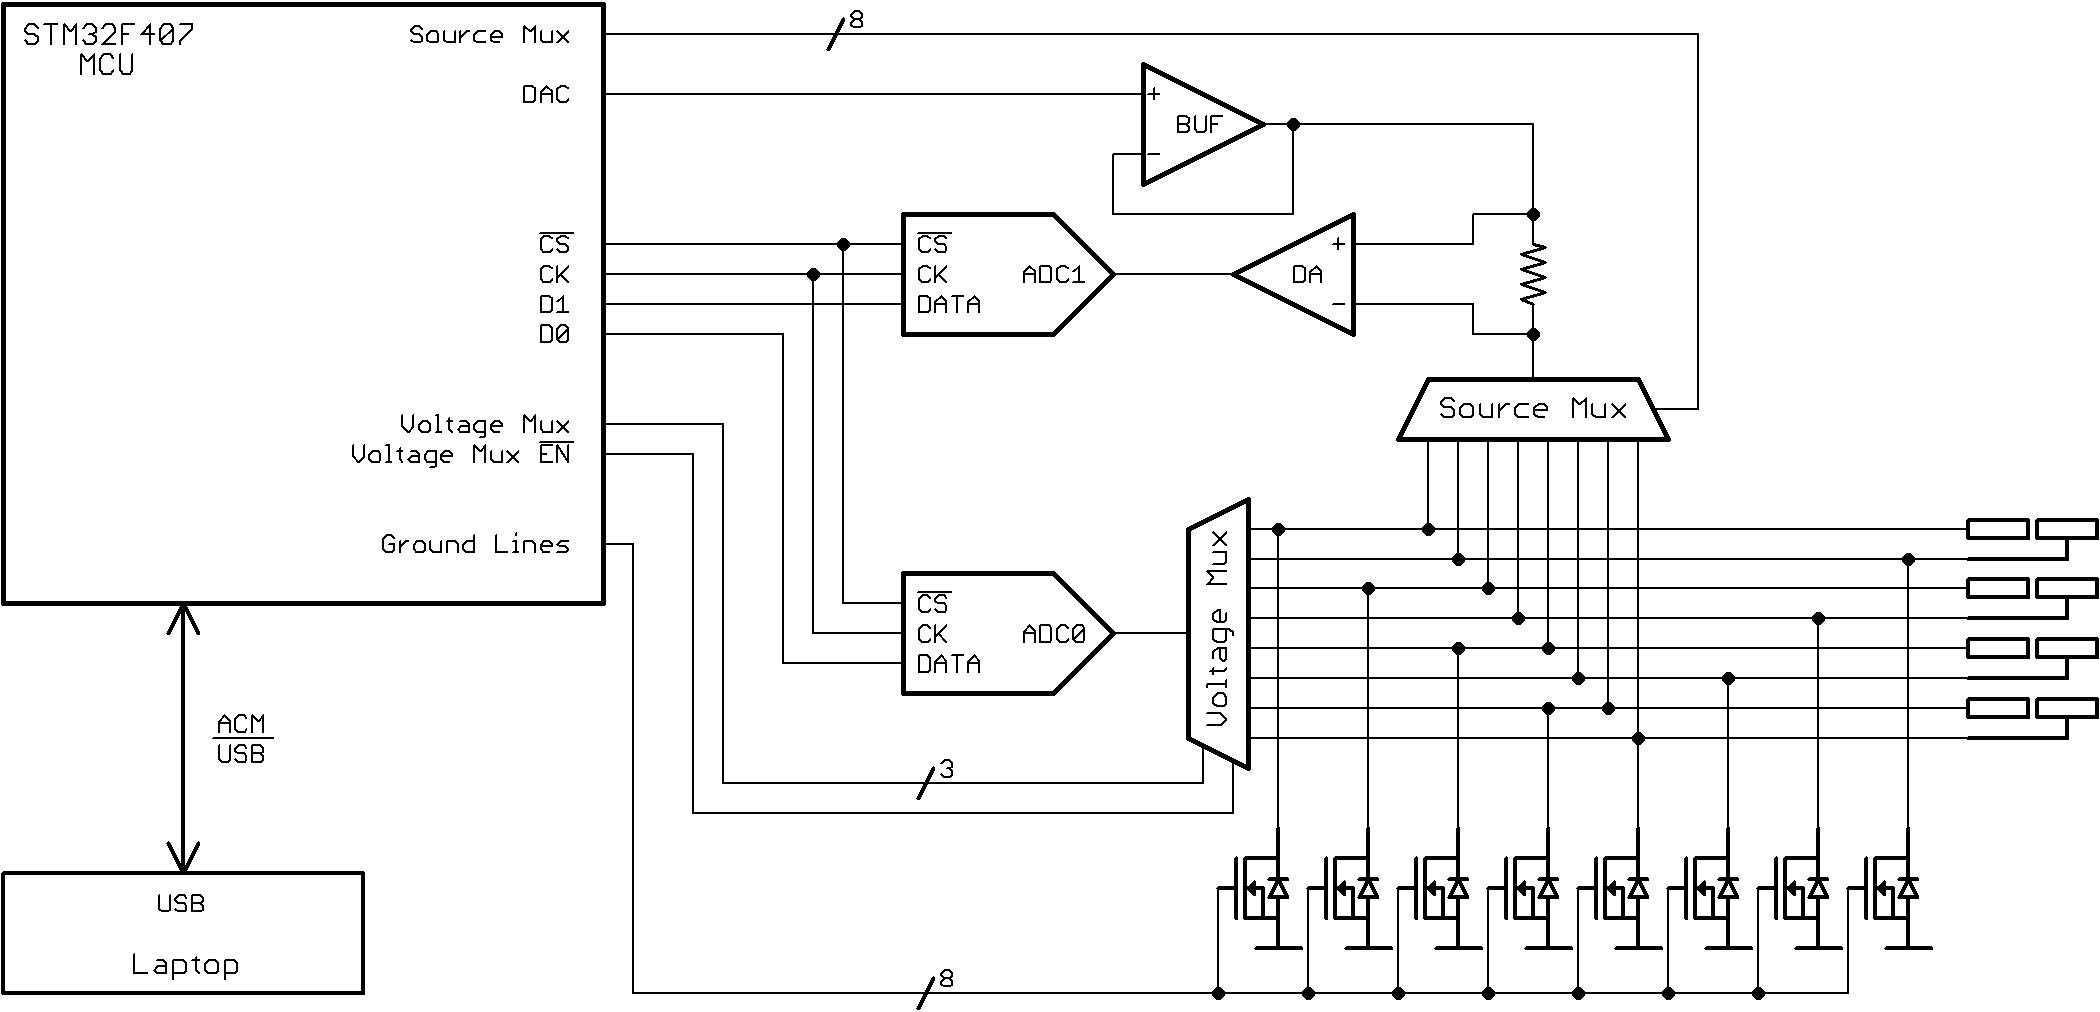
\includegraphics[width=1\textwidth]{../circuit.png}
  \end{center}
\end{figure}
\section{Low Cost}

Keeping the cost of production low makes butterboard accessible to the largest population of people.
Using multiplexed ADCs where possible keeps the cost down by reducing the quantity of high price-tag components, like ADCs.

\section{Node Voltage Reading}
ADC+multiplexer

\section{Signal Generator}
Vsource + buffer

\section{Test Voltage Current Sensing}
Diff amp + current sense + ADC

\section{High-side Switches}
hi
\section{Low-side Switches}
lo

\section{PCB Mounted Breadboard}

\section{Hardware Prototypes}
%\end{document}
